\section{Interface definition of obstacle model}

\subsection{Description of obstacles}

Every obstacle is represented by an instance of the \code{Obstacle}
class. The following attributes define an obstacle:

\begin{itemize}
\item Dimension (width and height)
\item Position (top left and bottom right corner)
\item Angle of rotation
\item Frequency-dependent attenuation factor
\end{itemize}

\subsection{Managing obstacles}

A global instance of \code{ObstacleControl} (cf.~\fref{fig:obstacles})
manages all defined obstacles. It provides methods to determine the
attenuation when a line connecting two points (e.g., the line-of-sight
between two nodes) intersects one or more obstacles
(\code{computeAttenuation}), and, if so, which obstacles are involved
(\code{getIntersectingObstacles}). The \code{Obstacles} type is
defined as a vector of \code{Obstacle} references. The method returns
references of intersecting obstacles in the \code{out} parameter.

\begin{figure}
  \centering
  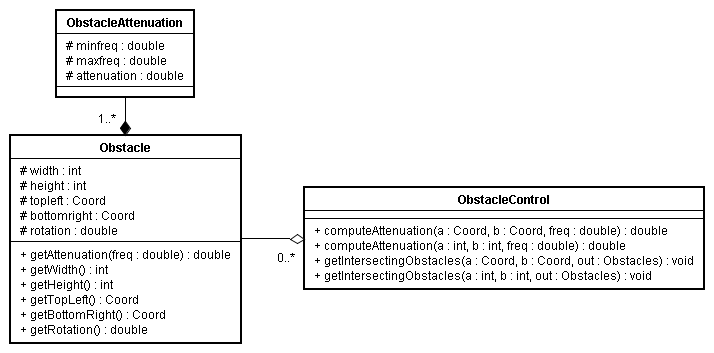
\includegraphics[scale=\scalefactor]{obstacles}
  \caption{Obstacles are managed by a global instance of
    ObstacleControl.}
  \label{fig:obstacles}
\end{figure}


\subsection{Interfacing the physical layer}

Simulations that intend to use obstacles, need to use the
\code{ObstacleFilter} (cf.~\fref{fig:filters}) that supplies the
additional attenuation caused by obstacles (if any) to the
\code{Signal}.  \code{ObstacleFilter} inherits from the
\code{AnalogueModel}, and it represents the interface that connects
the global instance of \code{ObstacleControl} to the physical layer
for computing additional attenuations.

\begin{figure}
  \centering
  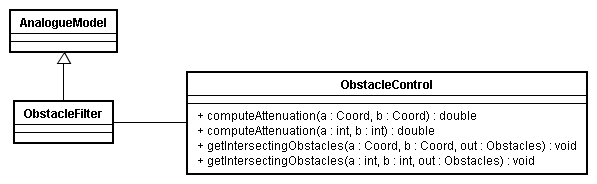
\includegraphics[scale=\scalefactor]{filters}
  \caption{The ObstacleFilter is an instance of AnalogueModel used for
    interfacing the physical layer.}
  \label{fig:filters}
\end{figure}


\subsection{Todos}

\begin{itemize}
\item How to implement mobility for obstacles?
\item How to associate nodes to obstacles?
\item How to return the length of intersections?
\end{itemize}



%%% Local Variables: 
%%% mode: latex
%%% TeX-master: "main"
%%% End: 
